\documentclass[10pt]{beamer}

\usetheme[progressbar=frametitle]{metropolis}
\usepackage{appendixnumberbeamer}
\usepackage{tikz}
\usepackage{tikzpeople}
\usetikzlibrary{shapes,fit}
\usepackage{xcolor}

\setbeameroption{hide notes} % Only slides
%\setbeameroption{show only notes} % Only notes
%\setbeameroption{show notes on second screen=right} % Both

\usepackage{amsmath}

\usepackage{booktabs}
\usepackage[scale=2]{ccicons}

\usepackage{environ}

\usepackage{pgfplots}
\usepgfplotslibrary{dateplot}

%rectangles around nodes
\usetikzlibrary{calc}

%right of=30mm of X
\usetikzlibrary{positioning}

\usepackage{xspace}
\newcommand{\themename}{\textbf{\textsc{metropolis}}\xspace}

\usepackage{hyperref}

\title{Meteor From Space}
\subtitle{Cryptographically Secure Steganography For Realistic Distributions}
% \date{\today}
\date{2022-05-16}
\author{Jeremy Boy}
\institute{Universität zu Lübeck}
% \titlegraphic{\hfill\includegraphics[height=1.5cm]{logo.pdf}}

\newsavebox\myboxa
\newsavebox\myboxb
\newlength\myhta
\newlength\mydpa
\newlength\myhtb
\newlength\mydpb
\newlength\maxht

\newcommand\CCCcolumns[3]{%
\begin{lrbox}{\myboxa}
  \begin{minipage}{0.3\linewidth}
  #1
  \end{minipage}%
\end{lrbox}%
\begin{lrbox}{\myboxb}
  \begin{minipage}{0.3\linewidth}
  #3
  \end{minipage}%
\end{lrbox}% 
\settoheight\myhta{\usebox\myboxa}%
\settodepth\mydpa{\usebox\myboxa}%
\addtolength\myhta{\mydpa}%
\settoheight\myhtb{\usebox\myboxb}%
\settodepth\mydpb{\usebox\myboxb}%
\addtolength\myhtb{\mydpb}%
\setlength\maxht{\myhta}%
\ifdim\myhtb>\myhta
  \setlength\maxht{\myhtb}%
\fi
\begin{minipage}[t][\maxht][c]{0.45\linewidth}
  #1
\end{minipage}\hfill
\begin{minipage}[t][\maxht][c]{0.1\linewidth}
  #2
\end{minipage}\hfill
\begin{minipage}[t][\maxht][c]{0.45\linewidth}
  #3
\end{minipage}%
}

\AtBeginSection{\frame{\sectionpage}}
%\AtBeginSection{}
%\AtBeginSubsection{\frame{\subsectionpage}}

\newcommand\blfootnote[1]{%
  \begingroup
  \renewcommand\thefootnote{}\footnote{#1}%
  \addtocounter{footnote}{-1}%
  \endgroup
}

\makeatletter
\newsavebox{\measure@tikzpicture}
\NewEnviron{scaletikzpicturetowidth}[1]{%
  \def\tikz@width{#1}%
  \def\tikzscale{1}\begin{lrbox}{\measure@tikzpicture}%
  \BODY
  \end{lrbox}%
  \pgfmathparse{#1/\wd\measure@tikzpicture}%
  \edef\tikzscale{\pgfmathresult}%
  \BODY
}
\makeatother

\begin{document}

    \maketitle

    
    \begin{frame}{Introduction}
        \centering
        \tikzstyle{component} = []
        \begin{tikzpicture}
            \node[alice, minimum width=1cm] (alice) {};
            \node[bob, minimum width=1cm, right= 4cm of alice, mirrored] (bob) {};
            \draw[->, thick] (alice) -- coordinate (aux) (bob);
            \node[below=1mm of aux] {c};
            \node[charlie, mirrored, minimum width=1cm, above=of aux] (eve) {};
            \draw[->,red, ultra thick] (eve)--(aux);
            \node[component, below left=1cm and 1mm of alice] (m_alice) {m};
            \node[component, below right=1cm and 1mm of alice] (k_alice) {k};
            \draw[->, thick] (m_alice) -- (alice);
            \draw[->, thick] (k_alice) -- (alice);
            \node[component, right=of bob] (m_bob) {m};
            \node[component, below=of bob] (k_bob) {k};
            \draw[->, thick] (bob) -- (m_bob);
            \draw[->, thick] (k_bob) -- (bob);
        \end{tikzpicture}
    \end{frame}
    
    \begin{frame}{Introduction}
        \centering
        \tikzstyle{component} = []
        \begin{tikzpicture}
            \node[alice, minimum width=1cm] (alice) {};
            \node[bob, minimum width=1cm, right= 4cm of alice, mirrored] (bob) {};
            \draw[->, thick] (alice) -- coordinate (aux) (bob);
            \node[below=1mm of aux] {c};
            \node[police, evil, mirrored, minimum width=1cm, above=of aux] (eve) {};
            \draw[->,red, ultra thick] (eve)--(aux);
            \node[component, below left=1cm and 1mm of alice] (m_alice) {m};
            \node[component, below right=1cm and 1mm of alice] (k_alice) {k};
            \draw[->, thick] (m_alice) -- (alice);
            \draw[->, thick] (k_alice) -- (alice);
            \node[component, right=of bob] (m_bob) {m};
            \node[component, below=of bob] (k_bob) {k};
            \draw[->, thick] (bob) -- (m_bob);
            \draw[->, thick] (k_bob) -- (bob);
        \end{tikzpicture}
    \end{frame}
    
    \begin{frame}{Introduction}
        \centering
        \tikzstyle{component} = []
        \begin{tikzpicture}
            \node[alice, minimum width=1cm] (alice) {};
            \node[bob, minimum width=1cm, right= 4cm of alice, mirrored] (bob) {};
            \draw[->, thick] (alice) -- coordinate (aux) (bob);
            \node[below=1mm of aux] (s) {c};
            \node[police, evil, mirrored, minimum width=1cm, above=of aux] (eve) {};
            \draw[->,red, ultra thick] (eve)--(aux);
            \node[component, below=of alice] (m_alice) {m};
            \node[component, color=orange, below=of alice, left=of m_alice] (c_alice) {$\mathcal{C}$};
            \node[component, below right=of alice, right=of m_alice] (k_alice) {k};
            \draw[->, thick] (m_alice) -- (alice);
            \draw[->, thick] (k_alice) -- (alice);
            \draw[->, thick, draw=orange] (c_alice) -- (alice);
            \node[component, right=of bob] (m_bob) {m};
            \node[component, below=of bob] (k_bob) {k};
            \draw[->, thick] (bob) -- (m_bob);
            \draw[->, thick] (k_bob) -- (bob);
        \end{tikzpicture}
    \end{frame}
    
    \begin{frame}{Introduction}
        \centering
        \tikzstyle{component} = []
        \begin{tikzpicture}
            \node[alice, minimum width=1cm] (alice) {};
            \node[bob, minimum width=1cm, right= 4cm of alice, mirrored] (bob) {};
            \draw[->, thick] (alice) -- coordinate (aux) (bob);
            \node[color=orange, below=1mm of aux] (s) {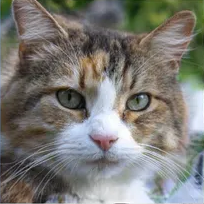
\includegraphics[width=30pt]{cat}};
            \node[police, evil, mirrored, minimum width=1cm, above=of aux] (eve) {};
            \draw[->,red, ultra thick] (eve)--(aux);
            \node[component, below=of alice] (m_alice) {m};
            \node[component, color=orange, below=of alice, left=of m_alice] (c_alice) {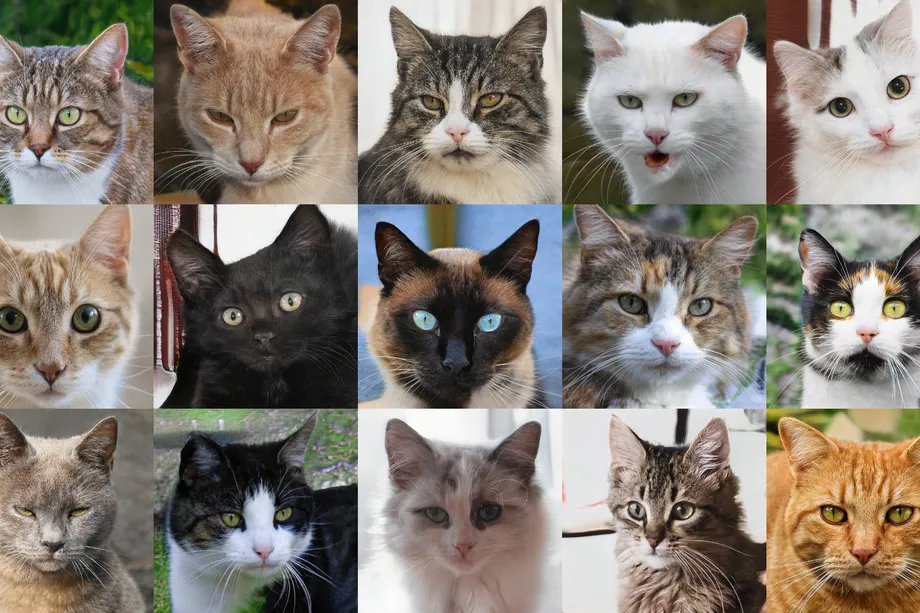
\includegraphics[width=60pt]{cats}};
            \node[component, below right=of alice, right=of m_alice] (k_alice) {k};
            \draw[->, thick] (m_alice) -- (alice);
            \draw[->, thick] (k_alice) -- (alice);
            \draw[->, thick, draw=orange] (c_alice) -- (alice);
            \node[component, right=of bob] (m_bob) {m};
            \node[component, below=of bob] (k_bob) {k};
            \draw[->, thick] (bob) -- (m_bob);
            \draw[->, thick] (k_bob) -- (bob);
        \end{tikzpicture}
    \end{frame}
    
    \begin{frame}{Meteor From Space}
      \setbeamertemplate{section in toc}[sections numbered]
      \tableofcontents[hideallsubsections]
    \end{frame}
    
    \section{Overview}
    
    \begin{frame}{Overview}
        \centering
        \begin{itemize}[<+- | alert@+>]
            \item Classical Steganography not applicable to realistic distributions
            \item Use \textit{generative approximation} of natural language to hide information
            \item Encrypt hiddentext $m$ using pre-shared key $k$ to get ciphertext $r$
            \item Alice: manipulate sampling from $\mathcal{C}$ using $r$ to create stegotext $s$
            \item Bob: recover $r$ from $s$ and decrypt $m$ using $k$
        \end{itemize}
        
    \end{frame}
    
    \section{Generative Neural Networks}
    
    \begin{frame}{Generative Neural Networks}
        \centering
        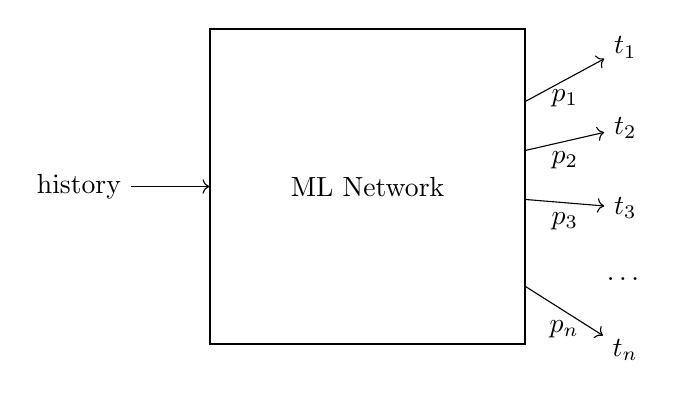
\begin{tikzpicture}
            \node[rectangle, draw=black, minimum width=4cm, minimum height=4cm] (oracle) {ML Network};
            \node[left=of oracle] (history) {history};
            \node[above right=-5mm and 1cm of oracle] (t1) {$t_1$};
            \node[below=5mm of t1] (t2) {$t_2$};
            \node[below=5mm of t2] (t3) {$t_3$};
            \node[below=5mm of t3] (t4) {$\dots$};
            \node[below=5mm of t4] (tn) {$t_n$};
            \draw[->] (history) -- (oracle);
            \draw[->] (oracle) -- node[midway,below] {$p_1$} (t1);
            \draw[->] (oracle) -- node[midway,below] {$p_2$} (t2);
            \draw[->] (oracle) -- node[midway,below] {$p_3$} (t3);
            %\draw[->] (oracle) -- (t4);
            \draw[->] (oracle) -- node[midway,below] {$p_n$} (tn);
        \end{tikzpicture}
    \end{frame}
       
    \begin{frame}{Generative Neural Networks}
        \centering
        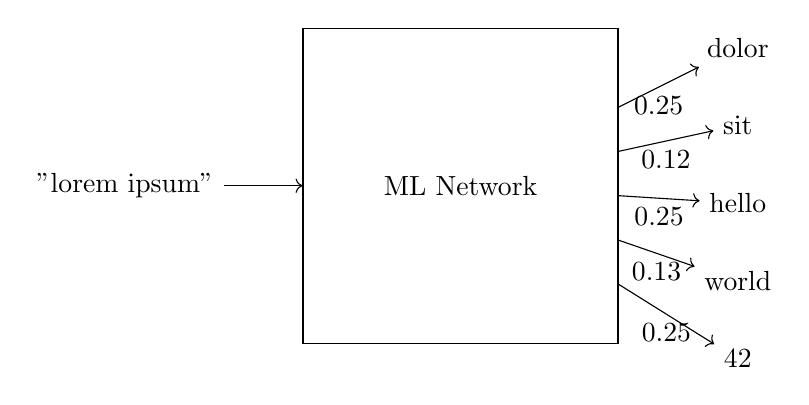
\begin{tikzpicture}
            \node[rectangle, draw=black, minimum width=4cm, minimum height=4cm] (oracle) {ML Network};
            \node[left=of oracle] (history) {"lorem ipsum"};
            \node[above right=-5mm and 1cm of oracle] (t1) {dolor};
            \node[below=5mm of t1] (t2) {sit};
            \node[below=5mm of t2] (t3) {hello};
            \node[below=5mm of t3] (t4) {world};
            \node[below=5mm of t4] (tn) {42};
            \draw[->] (history) -- (oracle);
            \draw[->] (oracle) -- node[midway,below] {0.25} (t1);
            \draw[->] (oracle) -- node[midway,below] {0.12} (t2);
            \draw[->] (oracle) -- node[midway,below] {0.25} (t3);
            \draw[->] (oracle) -- node[midway,below] {0.13} (t4);
            \draw[->] (oracle) -- node[midway,below] {0.25} (tn);
        \end{tikzpicture}
    \end{frame}
    
    \begin{frame}{Generative Neural Networks}
        \centering
        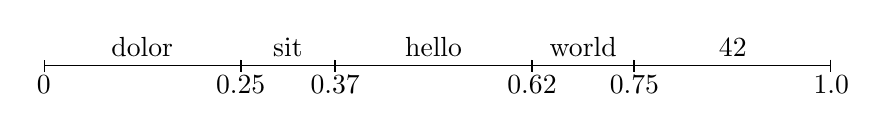
\begin{tikzpicture}
            \draw[|-|,fill=white] (0,0) node[below] {0} -- node[midway,above] {dolor} (2.5, 0);
            \draw[|-|,fill=white] (2.5,0) node[below] {0.25} -- node[midway,above] {sit} (3.7, 0);
            \draw[|-|,fill=white] (3.7,0) node[below] {0.37} -- node[midway,above] {hello} (6.2, 0);
            \draw[|-|,fill=white] (6.2,0) node[below] {0.62} -- node[midway,above] {world} (7.5, 0);
            \draw[|-|,fill=white] (7.5,0) node[below] {0.75} -- node[midway,above] {42} (10.0, 0) node[below] {1.0};
        \end{tikzpicture}
    \end{frame}
    
    \begin{frame}{Generative Neural Networks}
        \centering
        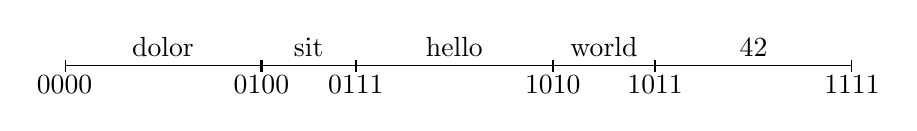
\begin{tikzpicture}
            \draw[|-|,fill=white] (0,0) node[below] {0000} -- node[midway,above] {dolor} (2.5, 0);
            \draw[|-|,fill=white] (2.5,0) node[below] {0100} -- node[midway,above] {sit} (3.7, 0);
            \draw[|-|,fill=white] (3.7,0) node[below] {0111} -- node[midway,above] {hello} (6.2, 0);
            \draw[|-|,fill=white] (6.2,0) node[below] {1010} -- node[midway,above] {world} (7.5, 0);
            \draw[|-|,fill=white] (7.5,0) node[below] {1011} -- node[midway,above] {42} (10.0, 0) node[below] {1111};
        \end{tikzpicture}
    \end{frame}
    
    \begin{frame}{Generative Neural Networks}
        \centering
        \begin{tikzpicture}
            \draw[|-|,fill=white] (0,0) node[below] {0000} -- node[midway,above] {dolor} (2.5, 0);
            \draw[|-|,fill=white] (2.5,0) node[below] {0100} -- node[midway,above] {sit} (3.7, 0);
            \draw[|-|,fill=white] (3.7,0) node[below] {0111} -- node[midway,above] {hello} (6.2, 0);
            \draw[|-|,fill=white] (6.2,0) node[below] {1010} -- node[midway,above] {world} (7.5, 0);
            \draw[|-|,fill=white] (7.5,0) node[below] {1011} -- node[midway,above] {\textbf{42}} (10.0, 0) node[below] {1111};
            \node at (9.6, 2) {
\includegraphics[height=10pt]{dogecoin.jpg} 1110};
            \draw[->,draw=orange] (9.6, 1.8) -- (9.6, 0);
        \end{tikzpicture}
    \end{frame}
    
    \section{Ranged Randomness Recoverable Sampling Scheme (RRRSS)}
    
    \begin{frame}{Ranged Randomness Recoverable Sampling Scheme}
        \begin{itemize}[<+- | alert@+>]
            \item Let $\mathcal{D}$ be a probability distribution and $\beta \in \mathbb{N}$
            \item We call $(\mathcal{D}, \beta)$ a RRRSS on distribution $\mathcal{D}$ with precision $\beta$, if:
                \begin{enumerate}
                \item $\operatorname{Sample}^\beta_\mathcal{D}(\mathcal{H}, r) \rightarrow s$. On history $\mathcal{H}$ and randomness $r \in \{0, 1\}^\beta$ sample an output $s$ from $\mathcal{D}$
                \item $\operatorname{Recover}^\beta_\mathcal{D}(\mathcal{H}, s) \rightarrow \mathcal{R}$. On history $\mathcal{H}$ and sample $s$, output the set $\mathcal{R}$ of possible values for $r$\blfootnote{$\mathcal{R} := \{ r \in \{0,1\}^\beta | \operatorname{Sample}^\beta_\mathcal{D}(\mathcal{H}, r) = s\}$}
                \end{enumerate}
        \end{itemize}
    \end{frame}
    
    % sample
    \begin{frame}{Ranged Randomness Recoverable Sampling Scheme}
        \begin{minipage}[c][0.6\textheight][c]{\textwidth}%
            \centering%
            \only<2>{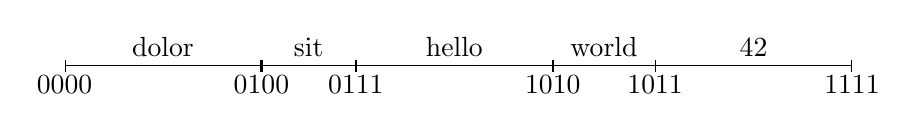
\begin{tikzpicture}
                \draw[|-|,fill=white] (0,0) node[below] {0000} -- node[midway,above] {dolor} (2.5, 0);
                \draw[|-|,fill=white] (2.5,0) node[below] {0100} -- node[midway,above] {sit} (3.7, 0);
                \draw[|-|,fill=white] (3.7,0) node[below] {0111} -- node[midway,above] {hello} (6.2, 0);
                \draw[|-,fill=white] (6.2,0) node[below] {1010} -- node[midway,above] {world} (7.5, 0);
                \draw[|-|,fill=white] (7.5,0) node[below] {1011} -- node[midway,above] {42} (10.0, 0) node[below] {1111};
            \end{tikzpicture}}%
            \only<3>{\begin{tikzpicture}
                \draw[|-|,fill=white] (0,0) node[below] {0000} -- node[midway,above] {dolor} (2.5, 0);
                \draw[|-|,fill=white] (2.5,0) node[below] {0100} -- node[midway,above] {sit} (3.7, 0);
                \draw[|-|,fill=white] (3.7,0) node[below] {0111} -- node[midway,above] {hello} (6.2, 0);
                \draw[|-,fill=white] (6.2,0) node[below] {1010} -- node[midway,above] {world} (7.5, 0);
                \draw[|-|,fill=white] (7.5,0) node[below] {1011} -- node[midway,above] {\textbf{42}} (10.0, 0) node[below] {1111};
                \node at (9.6, 2) {
\includegraphics[height=10pt]{dogecoin.jpg} 1110};
                \draw[->,draw=orange] (9.6, 1.8) -- (9.6, 0);
            \end{tikzpicture}}%
            \only<1-2>{$$\operatorname{Sample}^4_\mathcal{D}(\text{"lorem ipsum"}, 1110) =~ ?$$}%
            \only<3>{$$\operatorname{Sample}^4_\mathcal{D}(\text{"lorem ipsum"}, 1110) =~ \text{"42"}$$}%
        \end{minipage}%
        \vfill%
        \begin{minipage}[b][0.25\textheight][b]{\textwidth}%
            $\operatorname{Sample}^\beta_\mathcal{D}(\mathcal{H}, r) \rightarrow s$. On history $\mathcal{H}$ and randomness $r \in \{0, 1\}^\beta$ sample an output $s$ from $\mathcal{D}$
        \end{minipage}%
    \end{frame}
    
    % recover
    \begin{frame}{Ranged Randomness Recoverable Sampling Scheme}
        \begin{minipage}[c][0.6\textheight][c]{\textwidth}%
            \centering
            \only<2>{
                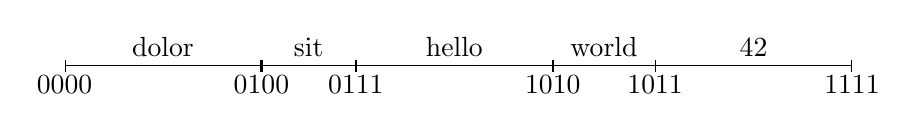
\begin{tikzpicture}
                    \draw[|-|,fill=white] (0,0) node[below] {0000} -- node[midway,above] {dolor} (2.5, 0);
                    \draw[|-|,fill=white] (2.5,0) node[below] {0100} -- node[midway,above] {sit} (3.7, 0);
                    \draw[|-|,fill=white] (3.7,0) node[below] {0111} -- node[midway,above] {hello} (6.2, 0);
                    \draw[|-,fill=white] (6.2,0) node[below] {1010} -- node[midway,above] {world} (7.5, 0);
                    \draw[|-|,fill=white] (7.5,0) node[below] {1011} -- node[midway,above] {42} (10.0, 0) node[below] {1111};
                \end{tikzpicture}
            }%
            \only<3>{
                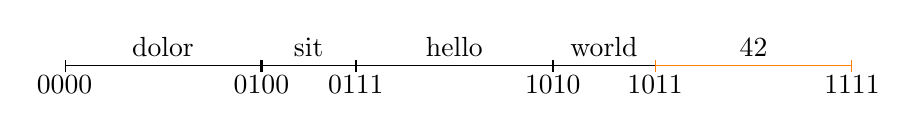
\begin{tikzpicture}
                    \draw[|-|,fill=white] (0,0) node[below] {0000} -- node[midway,above] {dolor} (2.5, 0);
                    \draw[|-|,fill=white] (2.5,0) node[below] {0100} -- node[midway,above] {sit} (3.7, 0);
                    \draw[|-|,fill=white] (3.7,0) node[below] {0111} -- node[midway,above] {hello} (6.2, 0);
                    \draw[|-,fill=white] (6.2,0) node[below] {1010} -- node[midway,above] {world} (7.5, 0);
                    \draw[|-|,draw=orange,fill=white] (7.5,0) node[below] {1011} -- node[midway,above] {42} (10.0, 0) node[below] {1111};
                \end{tikzpicture}
            }%
            \only<1-2>{$$\operatorname{Recover}^4_\mathcal{D}(\text{"lorem ipsum"}, \text{"42"}) =~ ?$$}
            \only<3>{\begin{align*}\operatorname{Recover}^4_\mathcal{D}(\text{"lorem ipsum"}, \text{"42"}) = \{ &1011, \\&1100, \\&1101, \\&1110, \\&1111 \}\end{align*}}
        \end{minipage}%
        \vfill%
        \begin{minipage}[b][0.25\textheight][b]{\textwidth}%
            $\operatorname{Recover}^\beta_\mathcal{D}(\mathcal{H}, s) \rightarrow \mathcal{R}$. On history $\mathcal{H}$ and sample $s$, output the set $\mathcal{R}$ of possible values for $r$
        \end{minipage}%
    \end{frame}
    
    \section{From RRRSS To Stegosystem}
    
    \begin{frame}{From RRRSS To Stegosystem}
        \begin{itemize}[<+- | alert@+>]
            \item Use $m$ to determine randomness used in sampling
            \item Problem: $m$ might be biased and can be observed by Warden
            \item Solution: at each iteration, encrypt the next $\beta$ bits of $m$ using PRG to get random value $r = m_{\beta} \oplus \operatorname{PRG.next}(k)$
            \item Use $r$ to sample $s = \operatorname{Sample}_\mathcal{D}^\beta(\mathcal{H}, r)$
            \item We have hidden a prefix of $r$ (and therefore $m$) in $s$
            \item Use $\operatorname{Recover}^\beta_\mathcal{D}(\mathcal{H}, s) = R$, calculate prefix of $R$
            \item Decrypt $m$ from recovered bits using $k$
        \end{itemize}
    \end{frame}
        
    \begin{frame}{From RRRSS To Stegosystem}
        \centering
        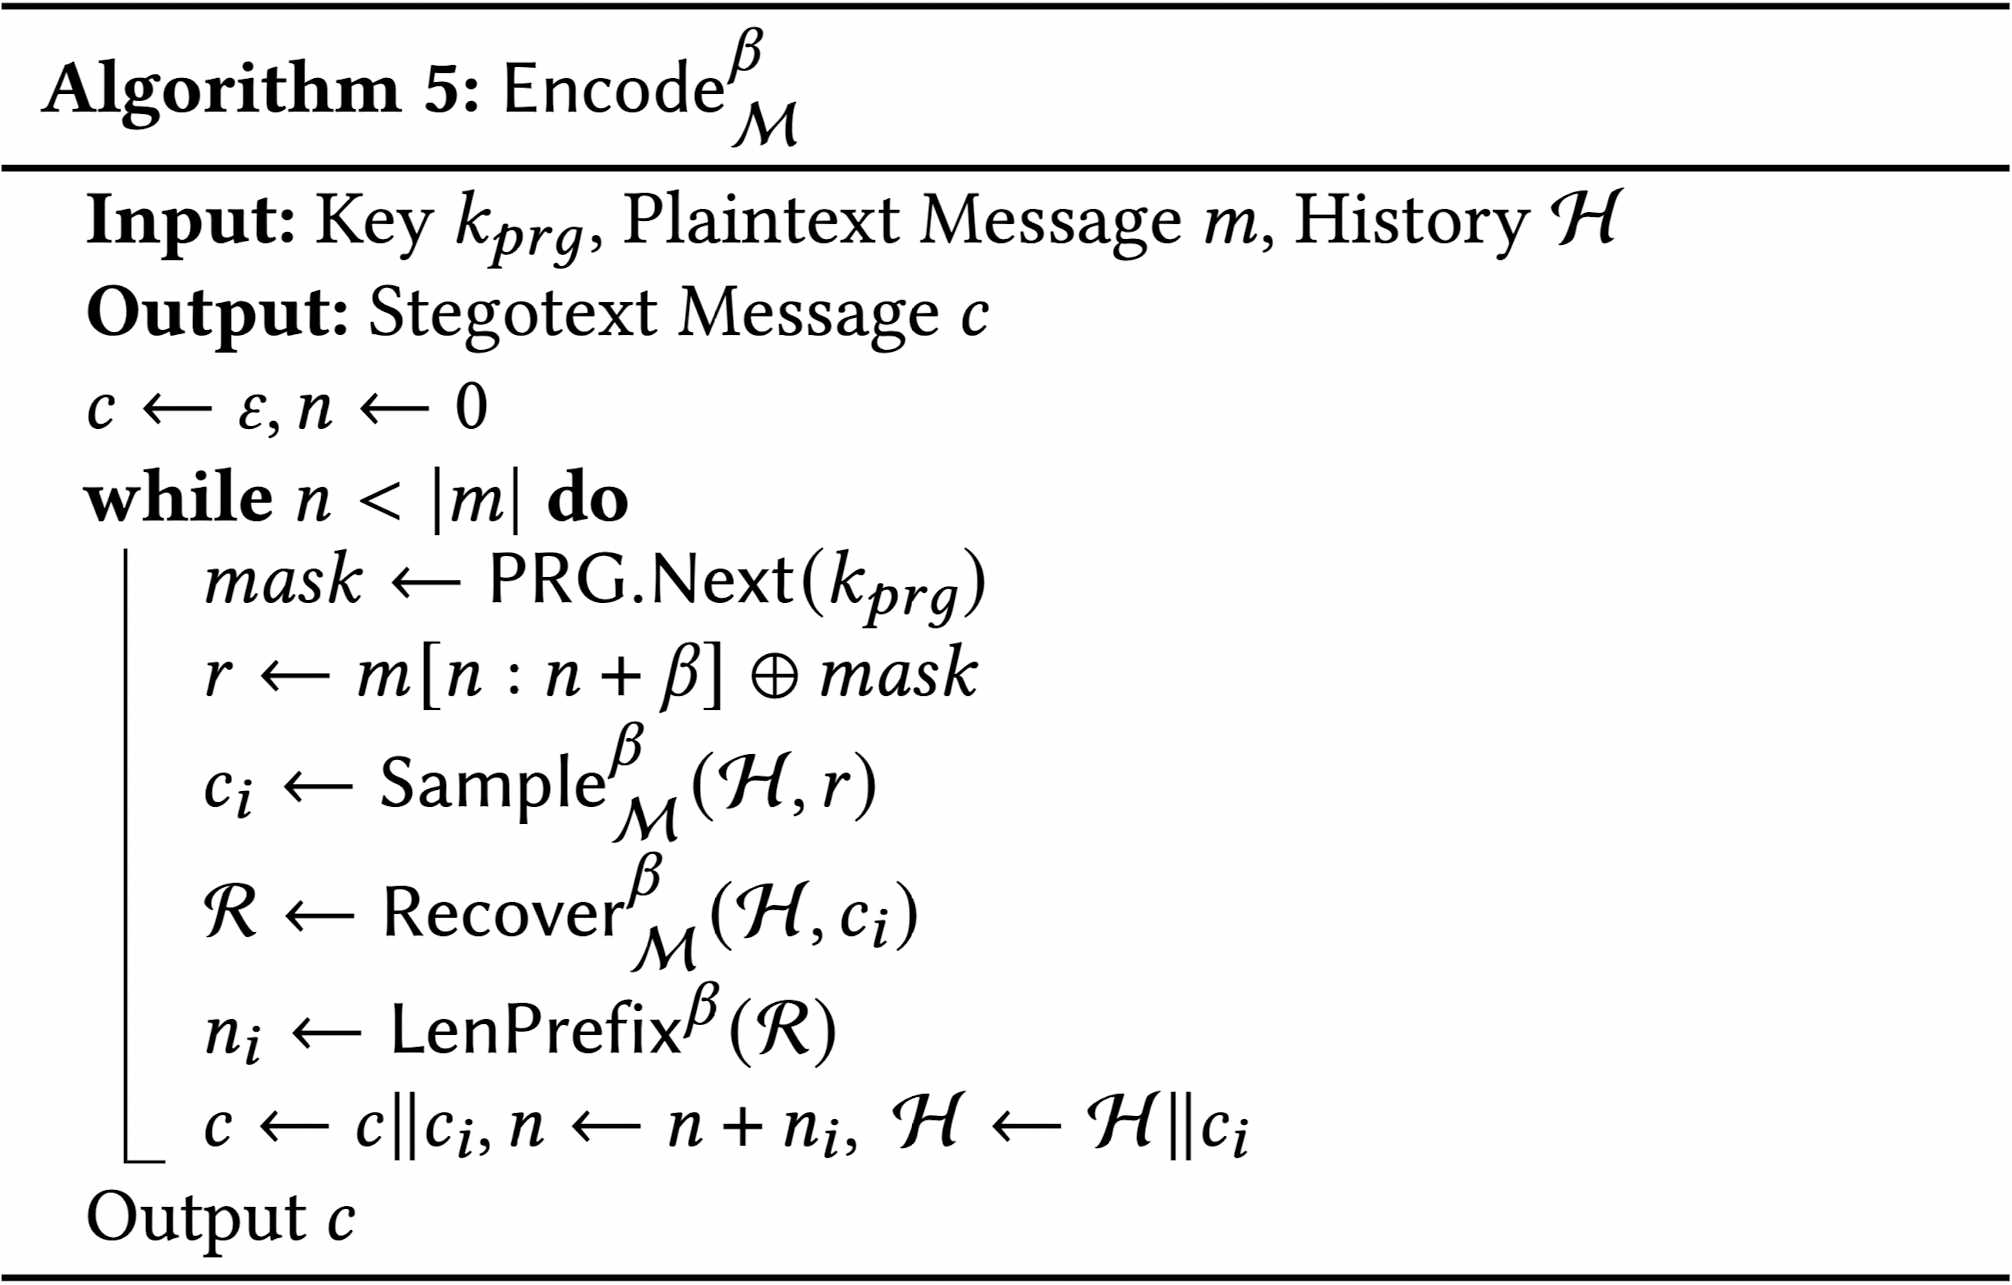
\includegraphics[width=0.9\textwidth]{alg-encode.png}
    \end{frame}
    
    \begin{frame}{From RRRSS To Stegosystem}
        \centering
        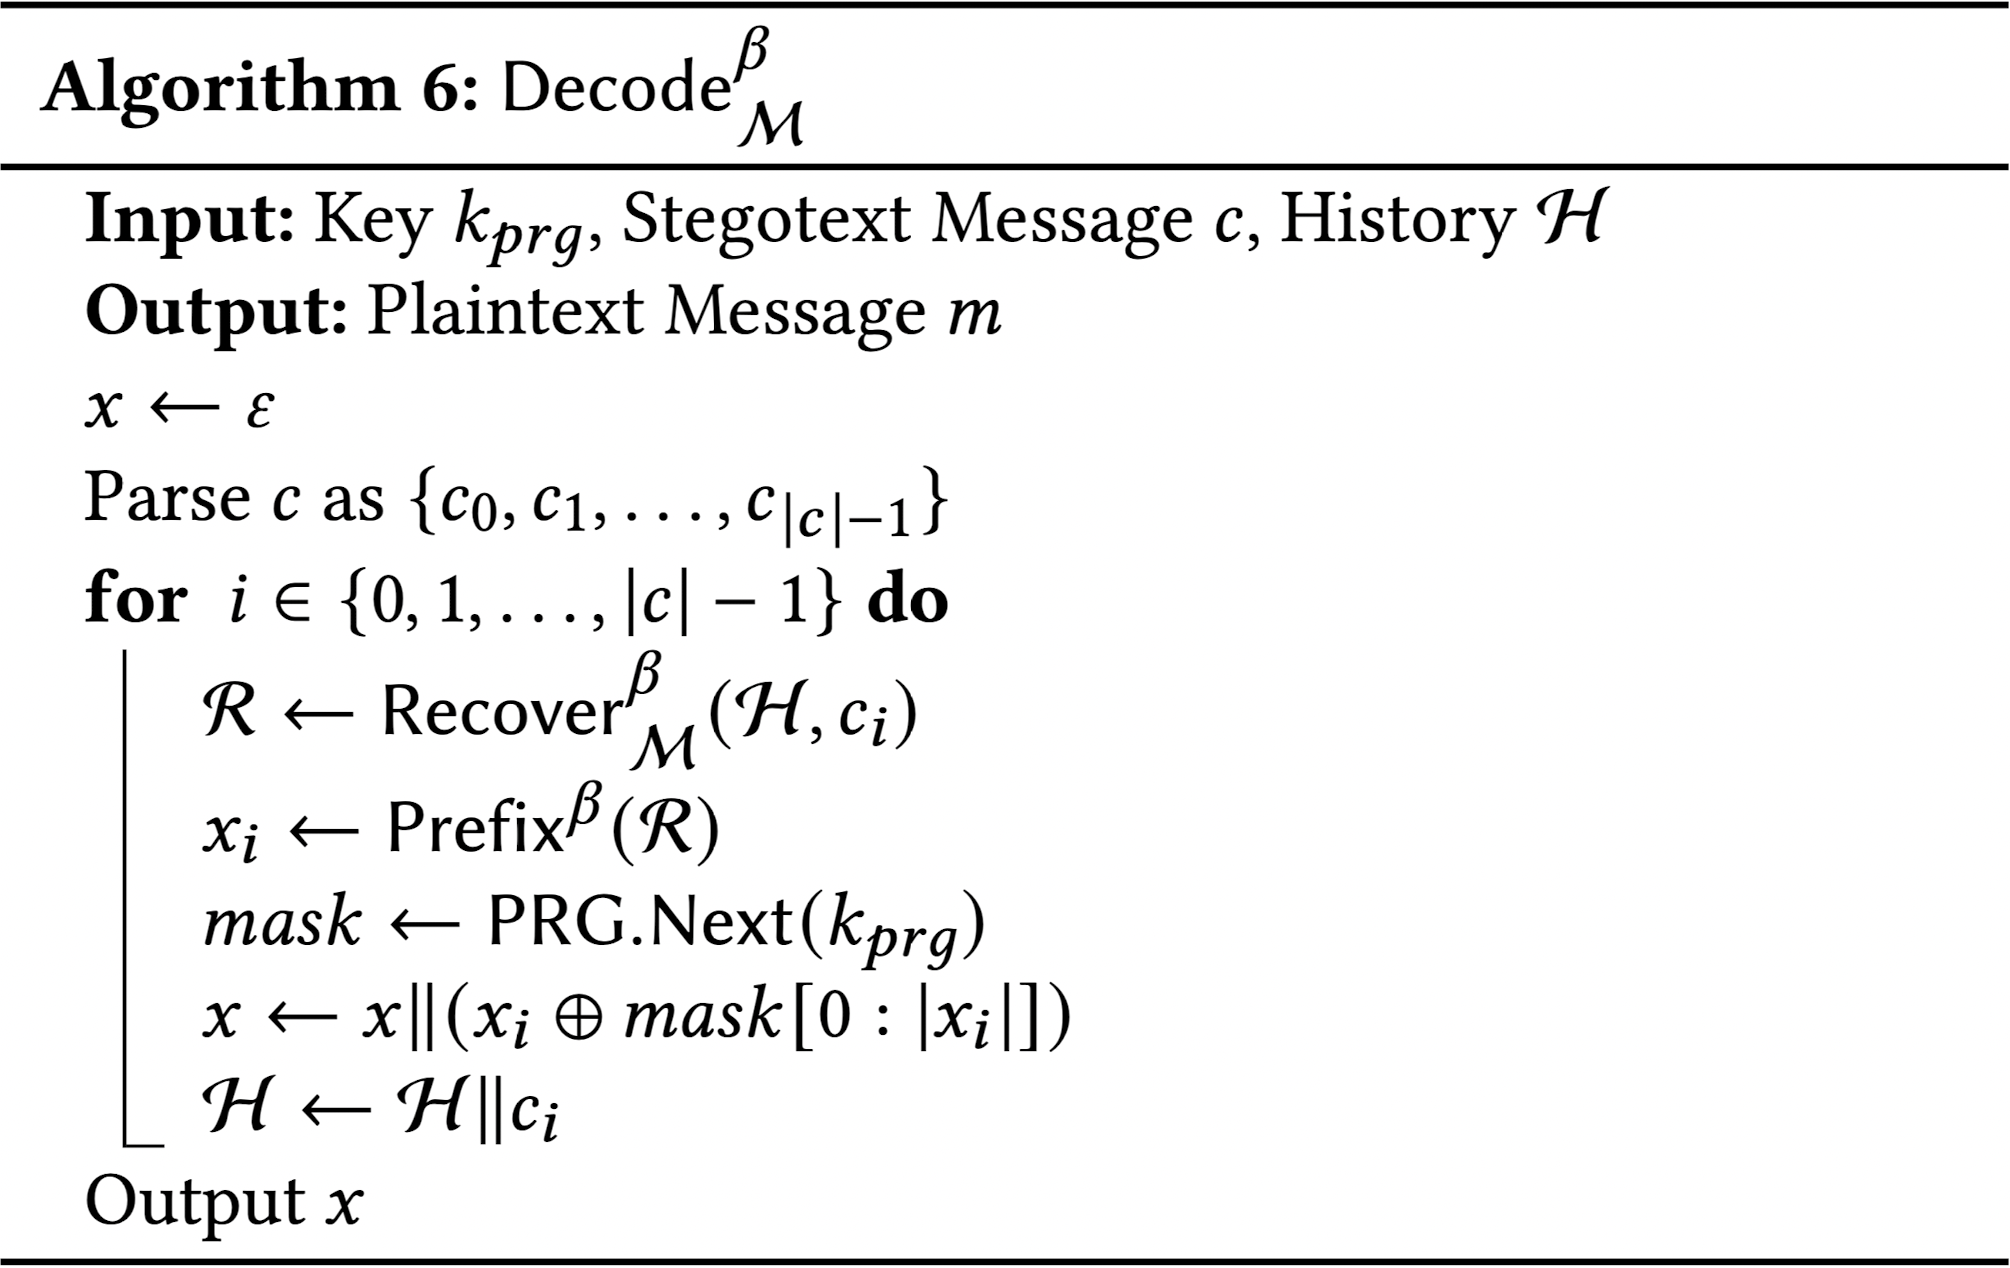
\includegraphics[width=0.9\textwidth]{alg-decode.png}
    \end{frame}
    
    \section{Security And Performance}
    
    \begin{frame}{Security And Performance}
        \begin{itemize}[<+- | alert@+>]
            \item Meteor proven secure (by reduction from PRG)
            \item Ca. 4 bits of hiddentext data per stegotext word
            \item Encoding/Decoding a 160 byte message takes:
                \begin{itemize}
                    \item 7 seconds on GPU (NVIDIA TITAN X)
                    \item 41 seconds on CPU (Intel Core i7-6700)
                    \item 473 seconds on Mobile (iPhone X)
                \end{itemize}
        \end{itemize}
    \end{frame}
    
    \section{Live Demo}
    
    \begin{frame}{Live Demo}
        \centering
        \href{https://colab.research.google.com/gist/tusharjois/ec8603b711ff61e09167d8fef37c9b86}{Meteor Live Demo}
    \end{frame}
    
    \section{Conclusion}
    
    \begin{frame}{Conclusion}
        \begin{itemize}[<+- | alert@+>]
            \item We can use generative neural networks to build cryptographically secure stegosystems
            \item Generated texts are hardly distinguishable from actual human texts (and will even become better)
            \item We can achieve competitive performance using symmetric encryption
        \end{itemize}
    \end{frame}
    
\end{document}